\section{Introduction}
\label{sec:intro}

\emph{The claim.}
An observer looks at a periodic pattern through a lens of finite resolution $\sigma$.
She may put her focus anywhere, and make it as narrow as the resolution allows or as wide as she likes.
This paper proves that no choice of focus helps her beyond a fixed rate.
\begin{quote}
\emph{Wherever the observer focuses, and however fine the resolution, the information that reaches her obeys $g\sqrt{\ell}\ge1-\bar\varepsilon$, with $\ell=\ln(1/\sigma)$.}
\end{quote}
The statement holds for every window whose ripple is weak in the sup norm, $\eta\le1/\ell$, for every state of such a window, and for every $\ell\ge55.26$, that is, for $\sigma\le e^{-55.26}\approx1.002\times10^{-24}$ with no lower limit on $\sigma$ (Theorem~\ref{thm:main}).
The constant $\bar\varepsilon$ bounds a remainder on the window class; it is the same constant as in Papers~F and~H~\cite{F,H}, and we do not improve it here.

\emph{Where this stands.}
Paper~F~\cite{F} introduced the quantity $g$, which measures how much ``information about the direction of time'' a window keeps under a blur of width $\sigma$, and proved the logarithmic law $g_{\min}\sqrt\ell\to$ (a number between $1-\bar\varepsilon$ and $1$) for windows with at most twenty harmonics or with strong damping.
The coefficient one is the exchange rate between fineness and blur.
Paper~H~\cite{H} removed the restriction on the number of harmonics on the lower side, for windows with a weak ripple, but only on a part of the map of states:
the focus had to span at least about $0.7$ ripple periods ($\tau\ge20$), and the resolution had to stay above $\sigma\approx10^{-417}$ ($\ell\le960.8$).
Paper~H listed what was missing, from the nearest restriction to the farthest: the states with a narrow focus, and the resolutions beyond $\ell=960.8$.
Both are closed here.

\emph{The map.}
A state is a choice of focus.
Its main coordinate is $B=b/\sigma^2=1/V$, the inverse variance of the focus along the ripple; $B$ runs from $0$ (a focus that spans arbitrarily many periods) to $e^{2\ell}$ (a focus as narrow as the resolution).
Figure~\ref{fig:map} shows the plane of $\ell$ and $B$.
Five theorems share it, and no state is left over (Table~\ref{tab:map}).
\begin{itemize}
\item \emph{Focus at the resolution} ($b\in(1/2,1]$; Theorem~\ref{thm:res}).
  At this narrowness the ripple can only darken the picture, because the window is non-negative.
  The two background terms survive untouched and $g$ stays of order one.
  This is not where the law is tight.
\item \emph{Narrow focus} (Theorem~\ref{thm:narrow}).
  The focus sees a short piece of the ripple.
  A local expansion around the focus, with every remainder explicit, and one hypothesis on the local brightness, which is a consequence of positivity, give the law with the factor $\sqrt{1+10/\ell}$.
\item \emph{Wide focus} (Theorem~\ref{thm:wide}).
  The same proof, with other constants, reaches every focus down to $B=8\ell+100$.
  Here the phase turns appreciably between the centre and the edge of the focus (a chirp), and this helps: the hardest states are the narrowest ones.
\item \emph{Very wide focus} (Theorem~\ref{thm:verywide}).
  The focus averages hundreds of periods and the local expansion is useless.
  Two elementary facts replace it; we describe them below.
  They use no bound on $\eta$, so this part of the map is settled for every window of the class, whatever the strength of its ripple.
\item \emph{Moderate resolution, focus wider than about $0.7$ periods}: Theorem~H1 of Paper~H.
\end{itemize}

\begin{figure}
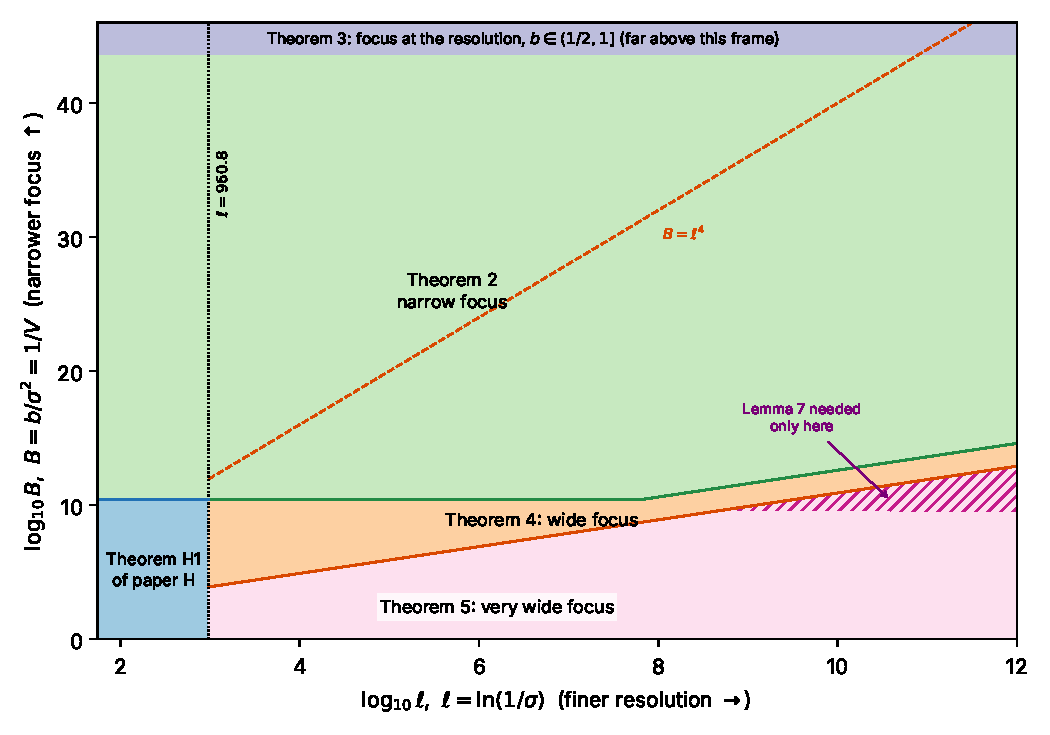
\includegraphics[width=\columnwidth]{figures/fig_map.pdf}
\caption{Which theorem covers which state. Horizontal axis: resolution, $\ell=\ln(1/\sigma)$. Vertical axis: narrowness of the focus, $B=b/\sigma^2$. The band at the top stands for $b\in(1/2,1]$, i.e.\ $B>e^{2\ell}/2$, which lies far above the frame. The region of Theorem~\ref{thm:verywide} continues below the frame down to $B\to0$. Hatched: the only states where Lemma~\ref{lem:P} is needed. The boundaries are the formulas of Table~\ref{tab:map}.}
\label{fig:map}
\end{figure}

\begin{table*}
\caption{The five theorems that cover the map, for windows with $\eta\le1/\ell$ in the regime $5\times10^{11}\sigma^2\le x\le0.003$. ``New'' means proved in this paper. The status labels are those of Papers~F and~H: \emph{proof} is closed by formulas alone; \emph{computer-assisted} uses finitely many interval-arithmetic computations as part of the proof.}
\label{tab:map}
\begin{ruledtabular}
\small
\begin{tabular}{p{0.12\textwidth}p{0.08\textwidth}p{0.26\textwidth}p{0.16\textwidth}p{0.15\textwidth}p{0.11\textwidth}}
focus & $\ell$ & $B=b/\sigma^2$ & theorem & bound on $g\sqrt\ell/(1-\bar\varepsilon)$ & status\\ \hline
at the resolution & $\ge55.26$ & $e^{2\ell}/2<B\le e^{2\ell}$ & Theorem~\ref{thm:res} (new) & $\ge0.19\sqrt\ell$ & proof\\
narrow & $\ge55.26$ & $\max(2.5\times10^{10},50(8\ell+100))\le B\le e^{2\ell}/2$ & Theorem~\ref{thm:narrow} (new) & $\ge\sqrt{1+10/\ell}$ & computer-assisted\\
wider than $0.7$ periods & $[55.26,960.8]$ & $B<2.5\times10^{10}$ & Theorem~H1 of~\cite{H} & $\ge1$ & computer-assisted\\
wide & $\ge960.8$ & $8\ell+100\le B<\ell^4$ & Theorem~\ref{thm:wide} (new) & $\ge\sqrt{1+10/\ell}$ & computer-assisted\\
very wide & $\ge960.8$ & $0<B\le8\ell+100$ & Theorem~\ref{thm:verywide} (new) & $\ge\sqrt{1+10/\ell}$ & proof\\
\end{tabular}
\end{ruledtabular}
\end{table*}

\emph{The two facts behind the very wide focus.}
When the focus spans many periods the observer no longer sees single ripples; what reaches her is the brightness averaged over a period.
The information she gets is the information in the slope of the ripple, multiplied by the phase mismatch between the centre and the edge of the focus, and the mismatch is as large as the focus is wide.
\begin{itemize}
\item \emph{Mean square instead of sup} (Proposition~\ref{prop:BE}).
  The enemy is a cross term between the curvature of the ripple and the phase mismatch.
  Paper~H measured it in mean square over the ripple rather than at its worst point, and used this only at the edge $B\le10^4$.
  We show that the heart of that argument depends neither on $B$ nor on $\ell$: the cross term costs at most $8\%$ of the slope information, whatever the width of the focus.
  Only the bookkeeping of the exponentially small remainders had to be redone.
\item \emph{Positivity and periodicity} (Lemma~\ref{lem:P}).
  If the focus spans only a few periods, averaging is not available.
  But the window is periodic along the ripple.
  Suppose a steep slope sits exactly where the phase mismatch vanishes, so that nothing can be read from it.
  The same slope is present one period away, and two periods away, and there the mismatch does not vanish.
  Those neighbours lie in the tail of the focus and are dim, but brightness is never negative, so they cannot cancel anything; they only count for less.
  The law asks for an amount of information of the order of the resolution itself, and the dim neighbours provide far more than that.
\end{itemize}
The second fact uses nothing but the shape of the window and the sign of the integrand; it may be of use elsewhere.

\emph{What is proved and what is not.}
We keep the distinction of Papers~F and~H between proof, computer-assisted proof, derivation, numerical evidence and conjecture, and mark every statement.
Table~\ref{tab:map} shows the status of the five theorems at a glance: two are proofs in the strict sense, three are computer-assisted.
The computer-assisted part consists of finitely many interval-arithmetic evaluations of explicit constants and conditions, with outward rounding, and of the certificates of Paper~H; it is listed in App.~\ref{app:C} and Table~\ref{tab:ca}.
We tried to break every claim before proving it.
For each one we report the families searched, the planted adversaries, and deliberately wrong versions that the same search does break (Sec.~\ref{sec:break}).
Direct two-dimensional quadrature reaches only $\ell\le10$, far from the range of the theorems; such comparisons are evidence about the formulas, not about the theorems, and are labelled \numst.

The limits of the result carry the same weight as the result.
\begin{itemize}
\item \emph{The window class.} The main theorem is for $\eta\le1/\ell$. Windows with a stronger ripple are outside it, except in two places: the very wide focus (Theorem~\ref{thm:verywide} needs no bound on $\eta$, so it holds for every window of the class), and the states of Paper~H's partial results. We make no claim beyond these.
\item \emph{The constant $\bar\varepsilon$.} Every bound carries the factor $1-\bar\varepsilon$ of condition (P6) of~\cite{F}. It is a hypothesis on the window class, not something we prove.
\item \emph{The regime.} We work in $5\times10^{11}\sigma^2\le x\le0.003$. The case $x\ge0.003$ is Theorem~48 of~\cite{F} (for $\sigma\le10^{-24}$); smaller $x$ is not treated.
\item \emph{The lower side only.} The upper side of the law is that of Paper~F and is not extended here.
\item \emph{Borrowed results.} Theorem~H1, the lower bound $g\ge(1-\bar\varepsilon)((a)+(a'))$, the brightness lemma CM-1, Lemma~R$_\theta$ and the mean-square step are taken from Papers~F and~H; the local lemmas behind the lines are new (App.~\ref{app:A}). Section~\ref{sec:main} says exactly which statement is borrowed and which is new.
\end{itemize}

\emph{Picture.}
A lens cannot be fooled by where it is pointed.
Narrow the focus to the resolution, and the background alone carries the information.
Widen it over hundreds of ripples, and the turning of the phase across the focus carries it.
In between, a short piece of ripple and the chirp share the load.
In every case what survives the blur is at least the fraction $1/\sqrt\ell$.
